\documentclass[11pt,a4paper]{article}

\usepackage[T1]{fontenc}
\usepackage[utf8]{inputenc}
\usepackage[spanish,es-nodecimaldot,es-noshorthands]{babel}
\usepackage[sc]{mathpazo}
\linespread{1.05}
\usepackage{amsmath,amssymb}
\usepackage{graphicx,subcaption,booktabs}
\usepackage{float}
\usepackage[margin=2.5cm]{geometry}
\usepackage{microtype}
\usepackage{titlesec}
\usepackage{fancyhdr}
\usepackage[font=small,labelfont=bf]{caption}
\usepackage[colorlinks=true, linkcolor=blue]{hyperref}


% Secciones con separador
\titleformat{\section}{\Large\bfseries}{\thesection.}{0.6em}{}[{\titlerule[0.6pt]}]
\titlespacing*{\section}{0pt}{1.6em}{0.9em}

% Encabezado
\pagestyle{fancy}
\fancyhf{}
\fancyhead[L]{\small\textsc{Macroeconomía Internacional Cuantitativa}}
\fancyhead[R]{\small Problem Set 3 --- Deuda con default}
\fancyfoot[C]{\small\thepage}
\renewcommand{\headrulewidth}{0.4pt}


\begin{document}

\begin{titlepage}
    \centering
    \vspace*{1cm}
    
\includegraphics[width=0.7\textwidth]{logo_udesa.pdf}\\[2cm]

    {\scshape\Large Maestría en Economía \par}
    \vspace{0.5cm}
    {\scshape\large Macroeconomía Internacional Cuantitativa \par}
    \vspace{1cm}

    \rule{\linewidth}{0.5pt}\\[0.4cm]
    {\huge\bfseries Problem Set 3\par}
    \vspace{0.1cm}
    {\Large Deuda con default\par}
    \rule{\linewidth}{0.5pt}\\[1cm]

    {\large
    Martín A. Fradkin \par}

    \vfill

    {\large Profesor: Francisco Roldán \par}
    \vspace{0.5cm}
    {\large \today \par}

\end{titlepage}

% ==================================================================
% INTRODUCCIÓN
% ==================================================================
\section*{Modelo y resolución numérica}
\label{sec:modelo}

Un soberano recibe un ingreso aleatorio $y$ y emite deuda de un período $b'$ a inversores extranjeros, al precio $q(b',y)$. En cada período, con deuda $b$ e ingreso $y$, elige entre repagar y entrar en default:
\begin{align}
\mathcal{V}(b,y) &= \max\big\{v^R(b,y)+\epsilon_R,\; v^D(y)+\epsilon_D\big\}, \label{eq:V}\\
v^R(b,y) &= \max_{b'}\; u\big(y-b+q(b',y)\,b'\big)+\beta\,\mathbb{E}\big[\mathcal{V}(b',y')\mid y\big], \label{eq:vR}\\
v^D(y) &= u\big(h(y)\big)+\beta\,\mathbb{E}\big[\psi\,\mathcal{V}(0,y')+(1-\psi)\,v^D(y')\mid y\big]. \label{eq:vD}
\end{align}
Los shocks $\epsilon_R$ y $\epsilon_D$ son iid con distribución de valor extremo tipo 1 y parámetro de escala $\chi$, de modo que
\begin{align}
\mathcal{P}(b,y)&=\frac{\exp\big(v^D(y)/\chi\big)}{\exp\big(v^R(b,y)/\chi\big)+\exp\big(v^D(y)/\chi\big)}, \label{eq:P}\\
\mathcal{V}(b,y)&=\chi\log\Big(\exp\big(v^D(y)/\chi\big)+\exp\big(v^R(b,y)/\chi\big)\Big), \label{eq:logsum}
\end{align}
donde $\mathcal{P}(b,y)$ es la probabilidad de default al llegar al estado $(b,y)$. Los acreedores son neutrales al riesgo y descuentan a la tasa $r$, por lo que el precio de la deuda es el repago esperado descontado:
\begin{equation}\label{eq:q}
q(b',y)=\frac{1}{1+r}\,\mathbb{E}\big[1-\mathcal{P}(b',y')\mid y\big].
\end{equation}

Se usa el código del curso (\texttt{arellano.jl}) con sus parámetros por defecto: $\beta=0.953$, $\gamma=2$ (utilidad CRRA), $r=0.017$, $\psi=0.282$, $\chi=0.01$, y un ingreso con $\log y$ AR(1) de persistencia $\rho_y=0.945$ y desvío $\sigma_y=0.025$. El costo de default es el original de Arellano (2008), $h(y)=\min\{y,\,y_h\}$ con $y_h=0.969$. La grilla de deuda tiene 200 puntos equiespaciados en $[0,\,0.6]$ y la de ingreso tiene 21 puntos entre $0.858$ y $1.165$ (método de Tauchen), con $y=1$ en el punto central.

El equilibrio se obtiene iterando en simultáneo sobre el precio \eqref{eq:q} y las funciones de valor \eqref{eq:V}--\eqref{eq:vD}, como en \texttt{mpe!}, hasta que la distancia relativa entre iteraciones sucesivas de $\mathcal{V}$ y de $q$ sea inferior a $10^{-6}$. El modelo base converge en 218 iteraciones. Para comparar regiones de default entre modelos se usa
\begin{equation}\label{eq:bstar}
b^\star(y):\quad \mathcal{P}\big(b^\star(y),\,y\big)=0.5,
\end{equation}
el nivel de deuda en el que la probabilidad de default cruza $50\%$ para cada ingreso, calculado por interpolación lineal de $\mathcal{P}$ entre los dos puntos de la grilla de $b$ que rodean el cruce.

% ==================================================================
\section{Deuda con default (Arellano)}
\label{sec:default}
% ==================================================================

\subsection{Regiones de repago y default}
\label{sec:regiones}

\begin{figure}[H]
\centering
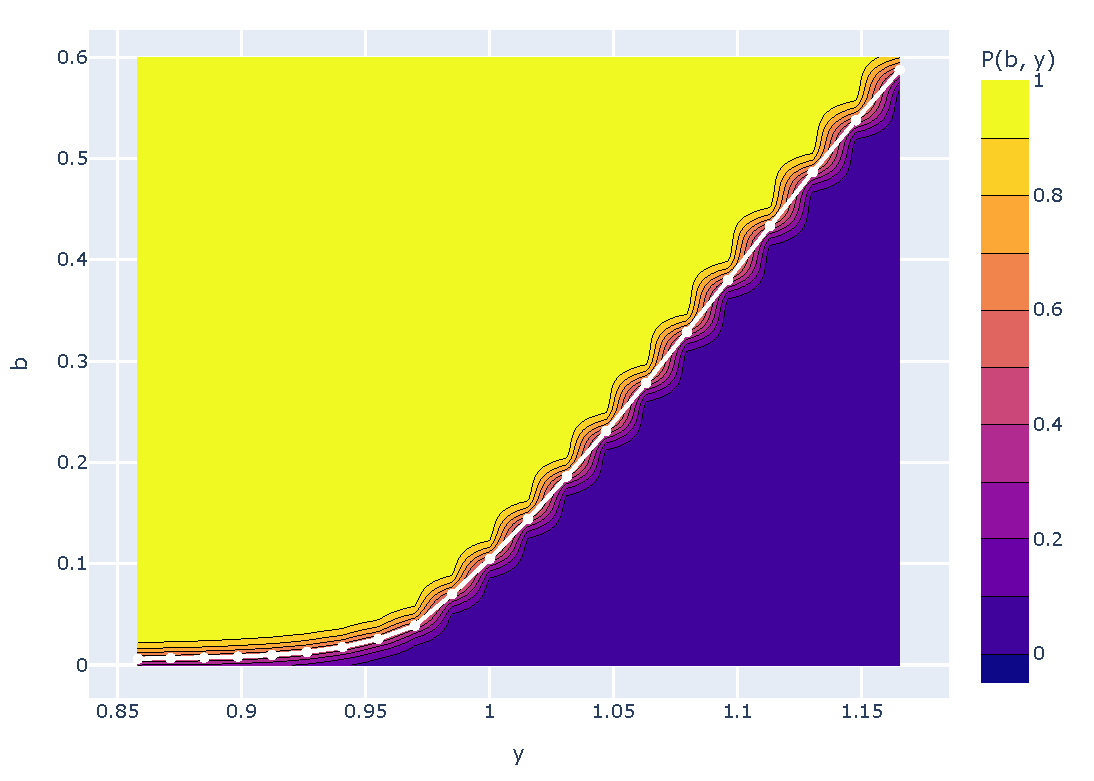
\includegraphics[width=0.7\textwidth]{prob_contour.pdf}
\caption{Probabilidad de default $\mathcal{P}(b,y)$ en el modelo base. La línea blanca es $b^\star(y)$, definido en \eqref{eq:bstar}.}
\label{fig:contour}
\end{figure}

\begin{table}[H]
\centering
\begin{tabular}{lccccc}
\toprule
$y$ & 0.858 & 0.926 & 1.000 & 1.079 & 1.165\\
\midrule
$b^\star(y)$ & 0.006 & 0.013 & 0.105 & 0.329 & 0.587\\
\bottomrule
\end{tabular}
\caption{Nivel de deuda en el que la probabilidad de default cruza $50\%$, modelo base.}
\label{tab:bstar}
\end{table}

La probabilidad de default crece con la deuda y cae con el ingreso en los 4200 puntos de la grilla (Figura~\ref{fig:contour}). La deuda sólo entra en el valor de repagar. Con más deuda el gobierno tiene que destinar más ingreso al repago, $v^R$ cae y $v^D$ no cambia, de modo que a partir de cierto nivel conviene defaultear. El ingreso actúa en sentido opuesto por dos vías. Un ingreso alto hace más fácil pagar hoy y, como el ingreso es persistente, anticipa ingresos altos en el futuro. Además, el ingreso que se pierde en default, $y-h(y)=\max\{0,\,y-y_h\}$, crece uno a uno con $y$ por encima de $y_h=0.969$, por lo que defaultear con ingreso alto cuesta más.

El segundo canal se ve en la forma de $b^\star(y)$. Con ingreso por debajo de $y_h$ el default no reduce el ingreso y su único costo es la exclusión del mercado, así que el gobierno defaultea con casi cualquier deuda. Entre $y=0.858$ e $y=0.970$, $b^\star(y)$ sube apenas de $0.006$ a $0.039$. Por encima de $y_h$ la pendiente es unas diez veces mayor, y $b^\star(y)$ pasa de $0.105$ en $y=1$ a $0.587$ en $y=1.165$ (Cuadro~\ref{tab:bstar}). Con deuda nula e ingreso bajo la probabilidad de default tampoco es cero ($0.296$ en $y=0.858$), por el shock de preferencias que se analiza en el inciso~\ref{sec:chi}.

La deuda es entonces más riesgosa cuando el ingreso es bajo, y en especial cuando cae por debajo de $y_h$. Los acreedores trasladan ese riesgo al precio. Con $y=1$, una emisión de $b'=0.1$ se coloca a $q=0.532$, contra $1/(1+r)=0.983$ sin riesgo, porque si el ingreso del período siguiente cae por debajo de $1$, esa deuda supera $b^\star(y')$ y el gobierno defaultea.

\subsection*{Opcional: paciencia y costo de default}

Se resolvió el modelo para seis valores de $\beta$ (con $y_h=0.969$) y para cinco valores de $y_h$ (con $\beta=0.953$), y en cada caso se calculó $b^\star(y)$. Como las curvas para distintos $\beta$ quedan superpuestas en niveles (Figura~\ref{fig:bstarbeta}a), la Figura~\ref{fig:bstarbeta}b muestra la diferencia de cada una con la del modelo base.

\begin{figure}[H]
\centering
\begin{subfigure}{.49\textwidth}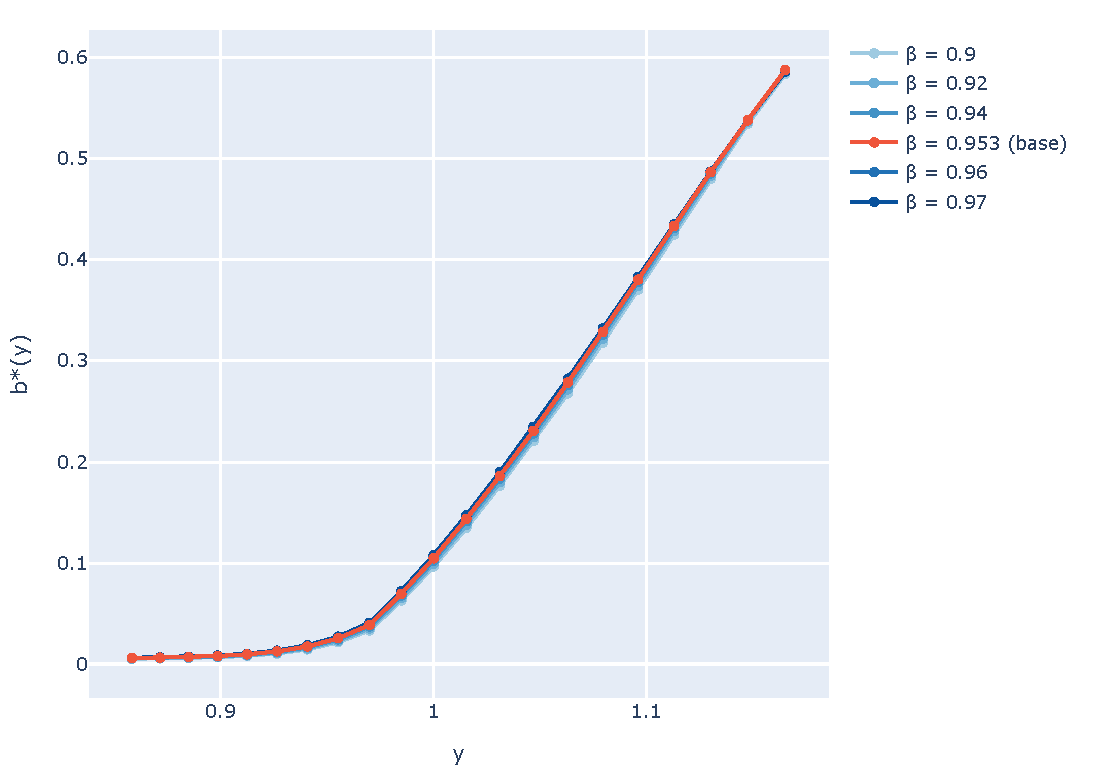
\includegraphics[width=\linewidth]{bstar_beta.pdf}\caption{$b^\star(y)$}\end{subfigure}
\begin{subfigure}{.49\textwidth}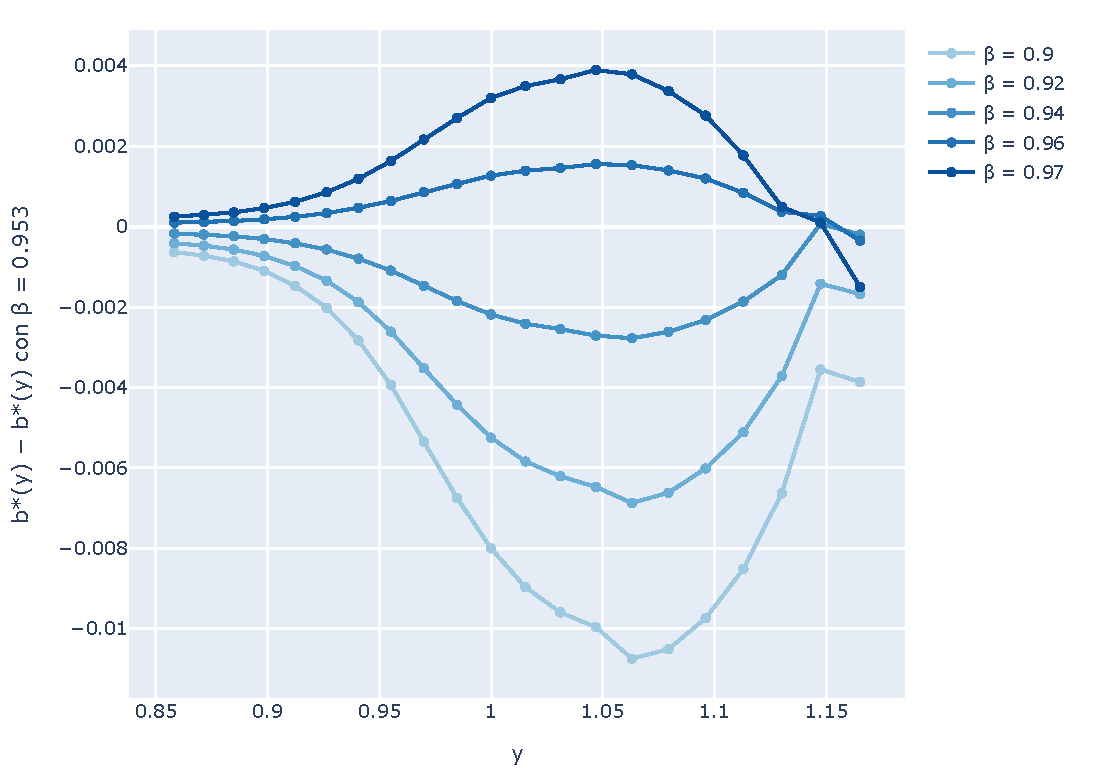
\includegraphics[width=\linewidth]{bstar_beta_dif.pdf}\caption{Diferencia con $\beta=0.953$}\end{subfigure}
\caption{$b^\star(y)$ para distintos valores del factor de descuento $\beta$, con $y_h=0.969$.}
\label{fig:bstarbeta}
\end{figure}

\begin{figure}[H]
\centering
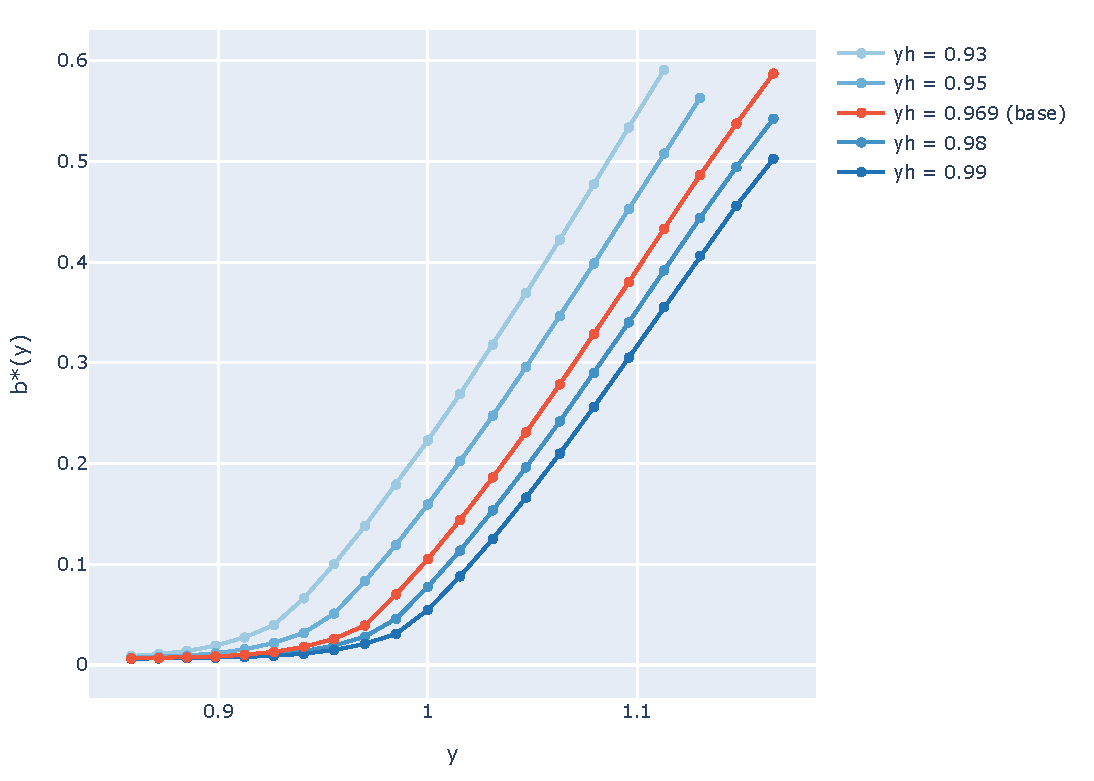
\includegraphics[width=0.6\textwidth]{bstar_yh.pdf}
\caption{$b^\star(y)$ para distintos valores de $y_h$, con $\beta=0.953$. Las curvas se cortan donde $b^\star(y)$ supera el máximo de la grilla de deuda, $0.6$.}
\label{fig:bstaryh}
\end{figure}

\begin{table}[H]
\centering
\begin{tabular}{lccccc}
\toprule
$y$ & 0.858 & 0.926 & 1.000 & 1.079 & 1.165\\
\midrule
$\beta=0.9$ & 0.006 & 0.011 & 0.097 & 0.318 & 0.584\\
$\beta=0.92$ & 0.006 & 0.012 & 0.100 & 0.322 & 0.586\\
$\beta=0.94$ & 0.006 & 0.012 & 0.103 & 0.326 & 0.587\\
$\beta=0.953$ (base) & 0.006 & 0.013 & 0.105 & 0.329 & 0.587\\
$\beta=0.96$ & 0.006 & 0.013 & 0.106 & 0.330 & 0.587\\
$\beta=0.97$ & 0.007 & 0.014 & 0.108 & 0.332 & 0.586\\
\midrule
$y_h=0.93$ & 0.009 & 0.039 & 0.223 & 0.477 & --\\
$y_h=0.95$ & 0.007 & 0.022 & 0.159 & 0.399 & --\\
$y_h=0.969$ (base) & 0.006 & 0.013 & 0.105 & 0.329 & 0.587\\
$y_h=0.98$ & 0.006 & 0.010 & 0.078 & 0.290 & 0.542\\
$y_h=0.99$ & 0.006 & 0.009 & 0.055 & 0.256 & 0.503\\
\bottomrule
\end{tabular}
\caption{$b^\star(y)$ para distintos $\beta$ (con $y_h=0.969$) y distintos $y_h$ (con $\beta=0.953$). ``--'': la probabilidad de default no llega a $50\%$ dentro de la grilla de deuda.}
\label{tab:bstaropc}
\end{table}

El costo de default mueve la región de default mucho más que la paciencia. Con $y=1$, $b^\star$ sube de $0.097$ a $0.108$ cuando $\beta$ pasa de $0.90$ a $0.97$, y de $0.055$ a $0.223$ cuando $y_h$ pasa de $0.99$ a $0.93$ (Cuadro~\ref{tab:bstaropc}).

\paragraph{Paciencia.} Un gobierno más paciente le da más peso a la exclusión futura, que es lo que pierde al defaultear, y tolera algo más de deuda. Con $\beta$ menor que el del modelo base, $b^\star(y)$ es menor o igual en los 21 ingresos, y con $\beta$ mayor es mayor o igual en 20 de ellos (Figura~\ref{fig:bstarbeta}b). El efecto es chico porque $\beta$ multiplica el valor de continuación de las dos opciones. En la comparación entre $v^R$ y $v^D$ sólo pesa a través de la diferencia entre el futuro con acceso al mercado y el futuro excluido, mientras que el costo de repagar, entregar $b$ del ingreso de hoy, no se descuenta.

\paragraph{Costo de default.} $y_h$ cambia directamente el consumo en default. Un $y_h$ menor es un costo mayor, porque el gobierno pierde $y-y_h$ cuando $y>y_h$, hoy y en cada período de exclusión. Por eso el quiebre de $b^\star(y)$ descripto en el inciso~\ref{sec:regiones} se desplaza con $y_h$ (Figura~\ref{fig:bstaryh}). Con $y_h=0.93$, $b^\star$ ya sube de $0.039$ a $0.066$ entre $y=0.926$ e $y=0.941$. Con $y_h=0.99$, en cambio, sigue en $0.031$ en $y=0.985$.

\subsection{Opcional -- Mecánica de los shocks de preferencias}
\label{sec:chi}

Se resolvió el modelo con $\chi\in\{0.0001,\,0.1\}$, además del valor por defecto $\chi=0.01$. La Figura~\ref{fig:valores} muestra $\mathcal{V}$, $v^R$ y $v^D$ en función de la deuda con $y=1$ (punto 11 de la grilla de ingreso), para $b\leq0.4$.

\begin{figure}[H]
\centering
\begin{subfigure}{.49\textwidth}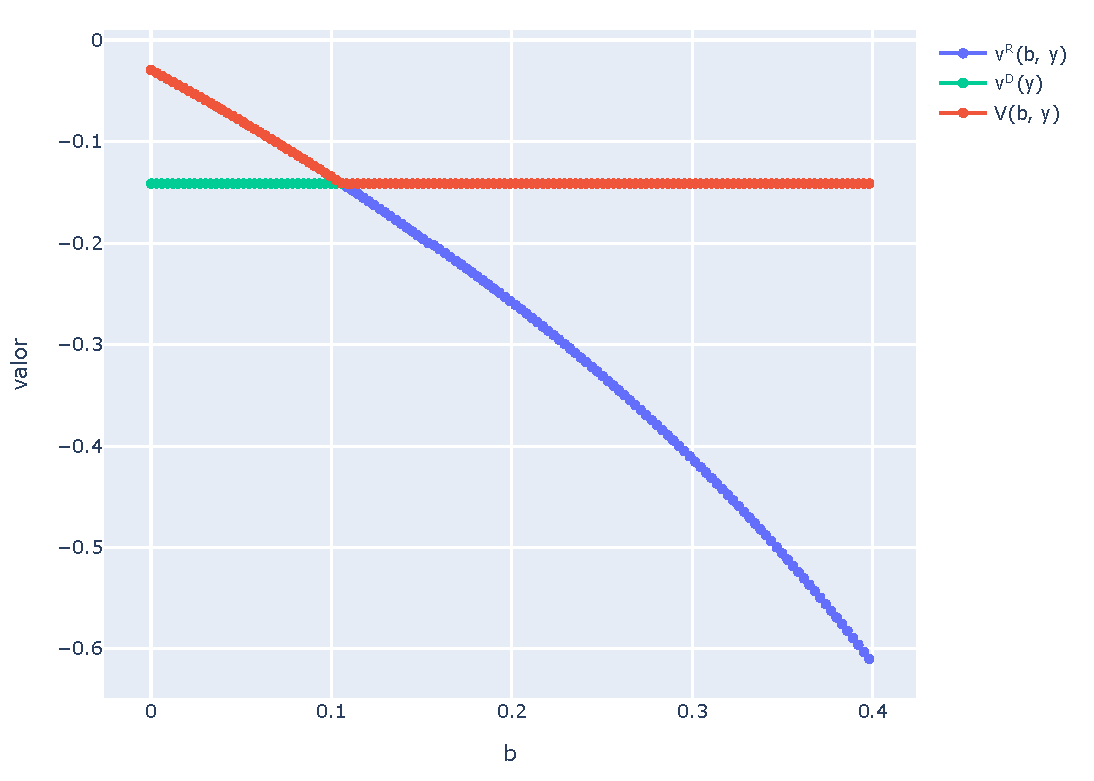
\includegraphics[width=\linewidth]{valores_chi_bajo.pdf}\caption{$\chi=0.0001$}\end{subfigure}
\begin{subfigure}{.49\textwidth}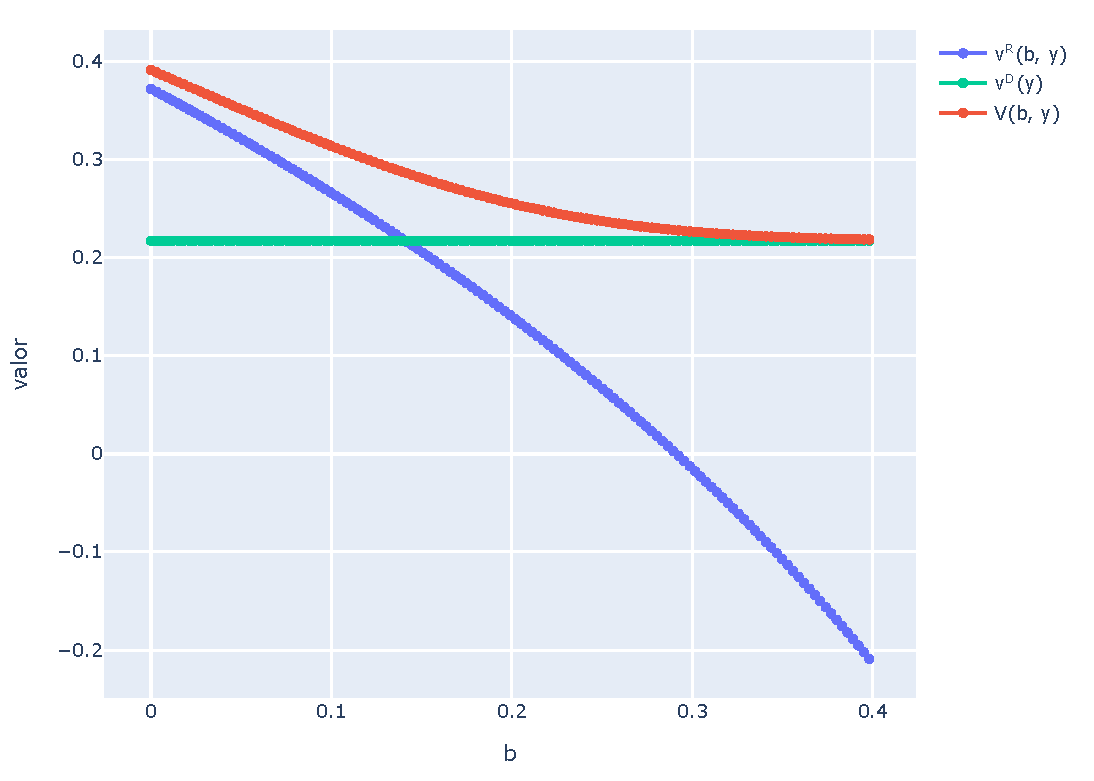
\includegraphics[width=\linewidth]{valores_chi_alto.pdf}\caption{$\chi=0.1$}\end{subfigure}
\caption{Funciones de valor $\mathcal{V}(b,y)$, $v^R(b,y)$ y $v^D(y)$ en $y=1$.}
\label{fig:valores}
\end{figure}

\begin{table}[H]
\centering
\begin{tabular}{lccc}
\toprule
 & $\chi=0.0001$ & $\chi=0.01$ & $\chi=0.1$\\
\midrule
$v^D(y)$                                   & $-0.1411$ & $-0.1337$ & $0.2170$\\
$v^R(0,y)$                                 & $-0.0291$ & $-0.0217$ & $0.3718$\\
$\mathcal{V}(0,y)$                         & $-0.0291$ & $-0.0217$ & $0.3911$\\
Deuda en la que $v^R=v^D$                  & $0.1058$  & $0.1049$  & $0.1409$\\
Máximo de $\mathcal{V}-\max\{v^R,v^D\}$    & $0.00001$ & $0.0066$  & $0.0688$\\
$\chi\log 2$                               & $0.00007$ & $0.0069$  & $0.0693$\\
$\mathcal{P}(0,y)$                         & $0.000$   & $0.000$   & $0.175$\\
\bottomrule
\end{tabular}
\caption{Funciones de valor en $y=1$ para distintos $\chi$. El máximo de $\mathcal{V}-\max\{v^R,v^D\}$ se toma sobre los 200 puntos de la grilla de deuda.}
\label{tab:chi}
\end{table}

\paragraph{Relación entre $\mathcal V$, $v^R$ y $v^D$.} La ecuación~\eqref{eq:logsum} puede escribirse como
\[
\mathcal V(b,y)=\max\{v^R,\,v^D\}+\chi\log\Big(1+e^{-|v^R-v^D|/\chi}\Big).
\]
El segundo término es el valor de elegir después de observar los shocks. Aunque $v^R<v^D$, un $\epsilon_R$ alto puede hacer que convenga repagar, y el gobierno se queda en cada realización con la mejor de las dos opciones. Ese término vale $\chi\log2$ cuando $v^R=v^D$, donde los shocks deciden la elección con probabilidad un medio, y tiende a cero cuando $|v^R-v^D|$ es grande respecto de $\chi$, porque entonces los shocks casi nunca cambian la elección. Con $\chi=0.0001$, $\mathcal V$ coincide con la envolvente $\max\{v^R,v^D\}$ y tiene un quiebre donde $v^R$ y $v^D$ se cruzan (Figura~\ref{fig:valores}a), con una diferencia máxima de $0.00001$. Con $\chi=0.1$, $\mathcal V$ es suave y queda por encima de las dos (Figura~\ref{fig:valores}b). La brecha llega a $0.0688$ cerca del cruce, casi $\chi\log2=0.0693$, y lejos de él se cierra. En $b=0.4$, $\mathcal V=0.2183$ y $v^D=0.2170$.

El shock también cambia la decisión. Con $\chi=0.1$ el gobierno defaultea con probabilidad $0.175$ aun sin deuda, porque $v^R(0,1)-v^D(1)=0.155$ no es grande respecto de $\chi$.

\paragraph{Niveles.} $\chi$ no da lo mismo para el valor del agente. Con $y=1$ y deuda nula, $\mathcal V$ vale $-0.0291$, $-0.0217$ y $0.3911$ para $\chi=0.0001$, $0.01$ y $0.1$ (Cuadro~\ref{tab:chi}). Tampoco $v^R$ y $v^D$ son iguales entre modelos, aunque $\chi$ no aparezca en \eqref{eq:vR} ni en \eqref{eq:vD}. Las dos tienen a $\mathcal V$ en el valor de continuación, y $\mathcal V$ incluye el valor de elegir en cada período futuro. Con $\chi=0.1$ ese valor es de hasta $0.0693$ por período, y descontado sobre un horizonte infinito de hasta $0.0693/(1-0.953)=1.47$. Cuanto mayor es $\chi$, más vale cada período futuro, y $v^R$ y $v^D$ suben juntas. $v^D(1)$ pasa de $-0.1337$ con $\chi=0.01$ a $0.2170$ con $\chi=0.1$.

\subsection{¿Cuántos defaults son por los precios?}
\label{sec:precios}

Se resolvió el problema del gobierno, con la opción de default, frente al precio $q=1/(1+r)=0.9833$ en toda la grilla: el precio de una deuda que se repaga siempre. Para eso se usó una variante de \texttt{mpe!} que no actualiza el precio con \eqref{eq:q}. La Figura~\ref{fig:precios} compara la región de default resultante con la del modelo base, y el Cuadro~\ref{tab:precios} cuenta los puntos de la grilla con $\mathcal{P}>0.5$ en cada modelo.

\begin{figure}[H]
\centering
\begin{subfigure}{.49\textwidth}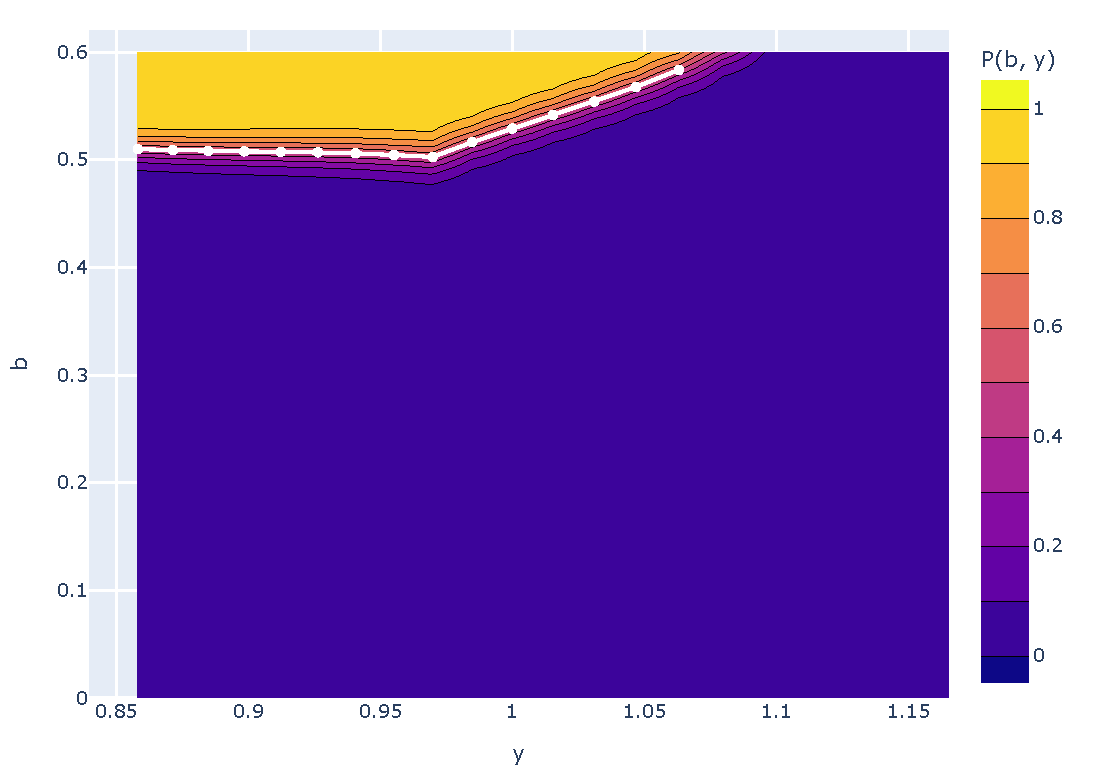
\includegraphics[width=\linewidth]{prob_contour_precios.pdf}\caption{$\mathcal{P}(b,y)$ con precios de repago seguro}\end{subfigure}
\begin{subfigure}{.49\textwidth}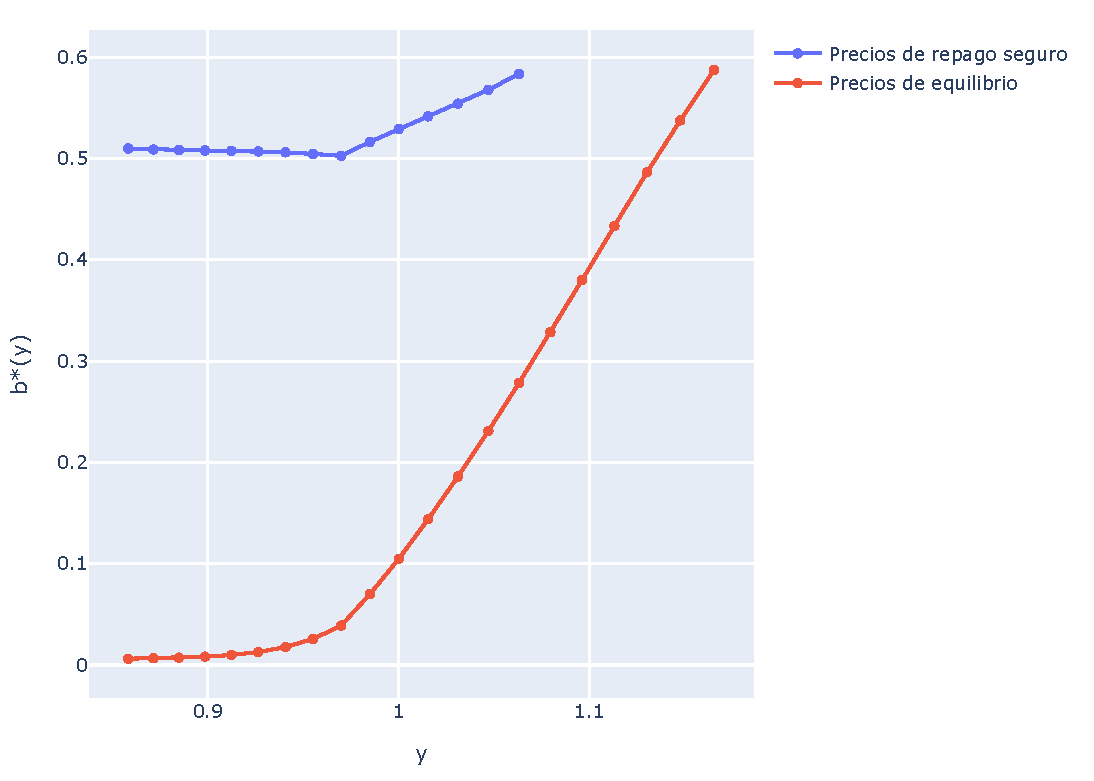
\includegraphics[width=\linewidth]{bstar_precios.pdf}\caption{$b^\star(y)$ en los dos modelos}\end{subfigure}
\caption{Región de default con precios de equilibrio y con precios de repago seguro. Con precios de repago seguro, $b^\star(y)$ supera el máximo de la grilla ($0.6$) para $y\geq1.079$.}
\label{fig:precios}
\end{figure}

\begin{table}[H]
\centering
\begin{tabular}{lc}
\toprule
 & Puntos $(b,y)$ con $\mathcal{P}>0.5$\\
\midrule
Precios de equilibrio              & 2896\\
Precios de repago seguro           & 387\\
\midrule
En ambos modelos                   & 387\\
Sólo con precios de equilibrio     & 2509\\
Sólo con precios de repago seguro  & 0\\
\midrule
Total de puntos de la grilla       & 4200\\
\bottomrule
\end{tabular}
\caption{Región de default ($\mathcal{P}>0.5$) en la grilla de $200\times21$ puntos.}
\label{tab:precios}
\end{table}

\begin{table}[H]
\centering
\begin{tabular}{lccccc}
\toprule
$y$ & 0.858 & 0.926 & 1.000 & 1.079 & 1.165\\
\midrule
Precios de equilibrio & 0.006 & 0.013 & 0.105 & 0.329 & 0.587\\
Precios de repago seguro & 0.510 & 0.507 & 0.529 & -- & --\\
Precios de repago seguro, $\bar b=1.2$ & 1.044 & 1.038 & 1.061 & 1.124 & 1.192\\
\bottomrule
\end{tabular}
\caption{$b^\star(y)$ con precios de equilibrio y con precios de repago seguro. La última fila repite el modelo de precios de repago seguro con una grilla de deuda en $[0,\,1.2]$. ``--'': la probabilidad de default no llega a $50\%$ dentro de la grilla.}
\label{tab:bstarprecios}
\end{table}

Las dos regiones son distintas, y la de precios de repago seguro es un subconjunto de la de equilibrio. Tiene 387 puntos de la grilla contra 2896, y ninguno queda fuera de la región de equilibrio (Cuadro~\ref{tab:precios}). Además, la probabilidad de default con precios fijos es menor que la de equilibrio en los 4200 puntos. Para $y\leq1.063$, $b^\star(y)$ va de $0.006$ a $0.279$ con precios de equilibrio y queda entre $0.503$ y $0.584$ con precios de repago seguro (Cuadro~\ref{tab:bstarprecios}).

La diferencia está en lo que cuesta renovar la deuda. Con precios fijos, el gobierno que debe $b$ puede emitir $b'=b$ a $q=0.983$ y repagar entregando sólo $0.017\,b$ del ingreso de hoy. Con precios de equilibrio el precio cae con la deuda emitida, y emitir más recauda cada vez menos. Con $y=1$ y una deuda de $0.2$, renovarla a precios fijos deja un consumo de $1-0.2+0.983\times0.2=0.997$. A precios de equilibrio, emitir $b'=0.2$ recauda $0.082\times0.2=0.016$ y emitir $b'=0.1$ recauda $0.053$, y el consumo cae a $0.816$ o a $0.853$, por debajo de los $0.969$ que obtiene en default. Esa comparación deja de lado los valores de continuación, pero coincide con lo que resuelve el modelo. En ese estado el gobierno defaultea con probabilidad 1 a precios de equilibrio y con probabilidad 0 a precios fijos.

Hay defaults que sólo ocurren por los precios. Son los 2509 puntos (el $87\%$ de la región de equilibrio) en los que el gobierno repagaría si pudiera renovar su deuda sin prima de riesgo. Esos precios no son ajenos al gobierno, porque reflejan la probabilidad de que defaultee más adelante. Con mucha deuda e ingreso bajo, el gobierno enfrenta precios bajos porque es probable que defaultee, y defaultea porque enfrenta precios bajos.

El ejercicio tiene un límite. Con precios fijos nada encarece la deuda, y el gobierno se endeuda hasta el máximo de la grilla ($b'=0.6$ para $b\geq0.1$ con $y=1$). Su región de default depende entonces de ese máximo. Con una grilla de deuda hasta $1.2$, $b^\star(y)$ pasa a estar entre $1.03$ y $1.19$ (última fila del Cuadro~\ref{tab:bstarprecios}). La inclusión de una región en la otra se verificó con la grilla original.

\paragraph{Conclusión.} El gobierno defaultea cuando repagar le exige un recorte de consumo mayor que lo que pierde al quedar excluido. Por eso la deuda es más riesgosa con ingreso bajo, y sobre todo por debajo de $y_h$, donde el default no le cuesta ingreso. El costo de default mueve la región de default mucho más que la paciencia, porque cambia directamente el consumo en default, mientras que $\beta$ sólo pesa a través del futuro de cada opción. El shock de preferencias suaviza la decisión y agrega a $\mathcal V$ el valor de poder elegir, que llega a $v^R$ y $v^D$ a través del valor de continuación. Por último, la mayor parte de los defaults del equilibrio ocurre porque el riesgo de default encarece la renovación de la deuda. Con precios que ignoran ese riesgo, el $87\%$ de la región de default desaparece.

% ==================================================================
\section{Calibración del modelo de default}
\label{sec:calibracion}
% ==================================================================

\subsection{Distribución ergódica}
\label{sec:ergodica}

Para cada modelo resuelto se simularon 400 trayectorias de $11\,000$ trimestres con la función \texttt{simul}, partiendo de $b_0=0$ e $y_0=1$, y se descartaron los primeros $1000$ trimestres de cada una. Los momentos se calculan en cada trayectoria y luego se promedian entre las 400. A los tres momentos de la función \texttt{moments} (deuda sobre PBI anual, promedio y desvío estándar del spread anualizado, todos calculados en los períodos de repago) se agregaron la mediana del spread, la frecuencia de default (defaults nuevos por cada 100 años con acceso al mercado) y el porcentaje del tiempo en default. Al repetir todo con otra semilla, los tres momentos de \texttt{moments} cambian menos de $0.7\%$ en todos los modelos de esta sección.

\subsection{Paciencia}
\label{sec:mombeta}

\begin{figure}[H]
\centering
\begin{subfigure}{.325\textwidth}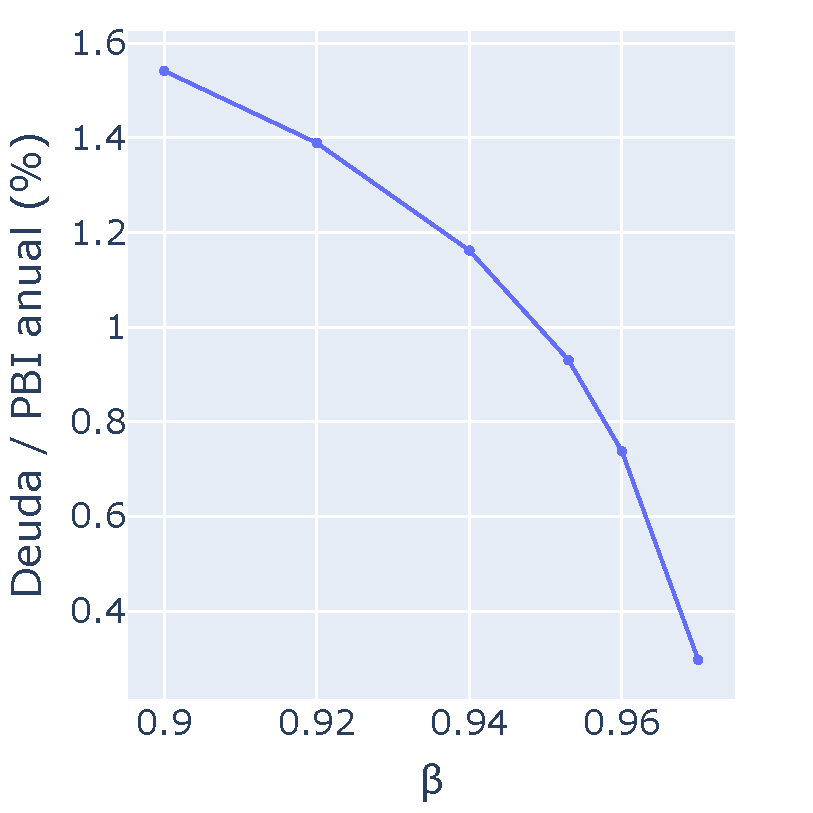
\includegraphics[width=\linewidth]{mom_deuda_beta.pdf}\caption{Deuda / PBI}\end{subfigure}
\begin{subfigure}{.325\textwidth}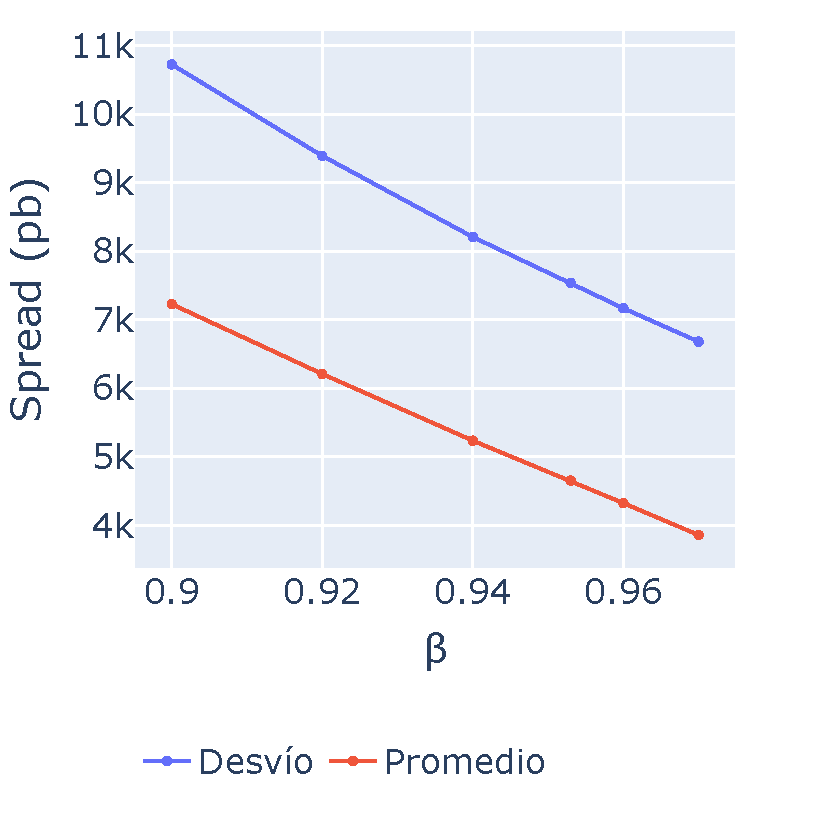
\includegraphics[width=\linewidth]{mom_spread_beta.pdf}\caption{Spread}\end{subfigure}
\begin{subfigure}{.325\textwidth}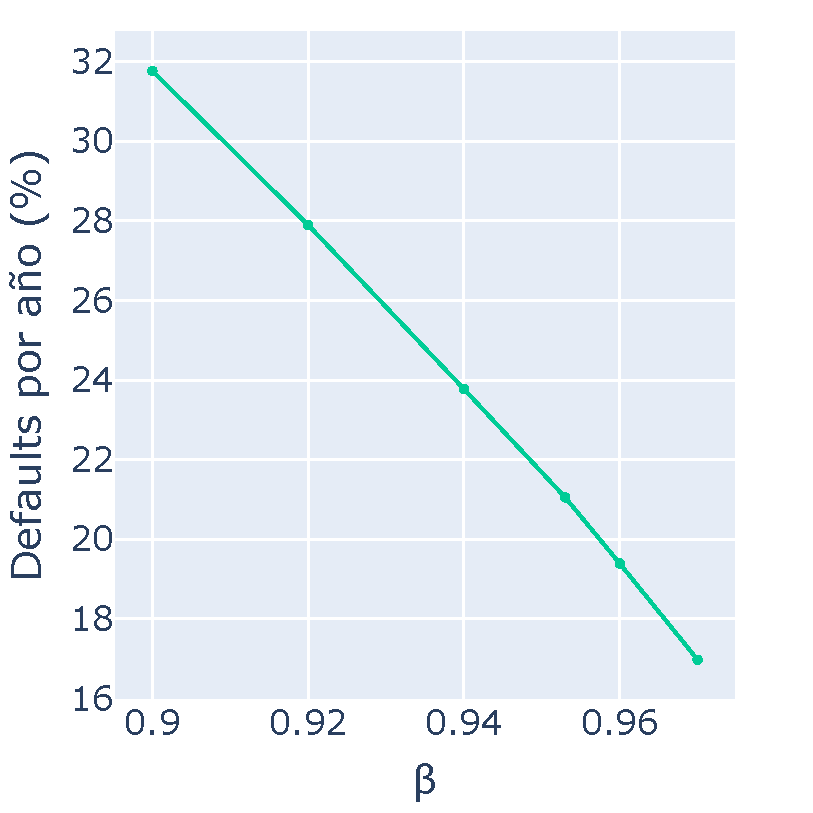
\includegraphics[width=\linewidth]{mom_def_beta.pdf}\caption{Frecuencia de default}\end{subfigure}
\caption{Momentos de la distribución ergódica en función de $\beta$, con $y_h=0.969$.}
\label{fig:mombeta}
\end{figure}

\begin{table}[H]
\centering
\begin{tabular}{lcccccc}
\toprule
 & Deuda/PBI & \multicolumn{3}{c}{Spread (puntos básicos)} & Defaults & Tiempo en\\
\cmidrule(lr){3-5}
 & (\%) & Promedio & Desvío & Mediana & por año (\%) & default (\%)\\
\midrule
$\beta=0.9$ & 1.54 & 7229 & 10725 & 3177 & 31.8 & 24.6\\
$\beta=0.92$ & 1.39 & 6211 & 9391 & 2628 & 27.9 & 22.3\\
$\beta=0.94$ & 1.16 & 5238 & 8208 & 2067 & 23.8 & 19.6\\
$\beta=0.953$ (base) & 0.93 & 4656 & 7540 & 1673 & 21.1 & 17.8\\
$\beta=0.96$ & 0.74 & 4327 & 7169 & 1446 & 19.4 & 16.6\\
$\beta=0.97$ & 0.30 & 3862 & 6682 & 1093 & 17.0 & 14.9\\
\bottomrule
\end{tabular}
\caption{Momentos de la distribución ergódica para distintos $\beta$, con $y_h=0.969$.}
\label{tab:mombeta}
\end{table}

Los cuatro momentos caen con $\beta$ en los seis valores (Figura~\ref{fig:mombeta} y Cuadro~\ref{tab:mombeta}). Entre $\beta=0.90$ y $\beta=0.97$, la deuda pasa de $1.54\%$ a $0.30\%$ del PBI anual, el spread promedio de 7229 a 3862 puntos básicos y la frecuencia de default de $31.8\%$ a $17.0\%$ por año. Un gobierno impaciente valora más el consumo de hoy y se endeuda más. Como $\beta$ casi no mueve la región de default (inciso~\ref{sec:regiones}), los gobiernos con distinto $\beta$ enfrentan casi los mismos precios, y el que se endeuda más queda más cerca de $b^\star(y)$. Paga entonces un spread más alto y defaultea con más frecuencia. La paciencia afecta el riesgo a través de la deuda que el gobierno elige, no del umbral en el que defaultea.

\subsection{Costos de default}
\label{sec:momyh}

\begin{figure}[H]
\centering
\begin{subfigure}{.325\textwidth}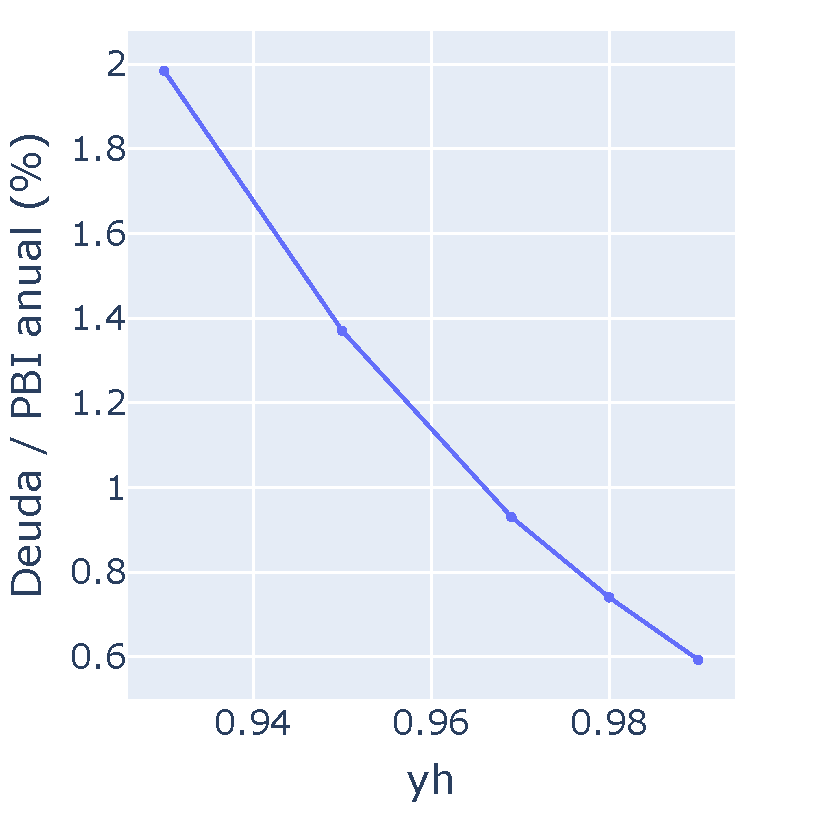
\includegraphics[width=\linewidth]{mom_deuda_yh.pdf}\caption{Deuda / PBI}\end{subfigure}
\begin{subfigure}{.325\textwidth}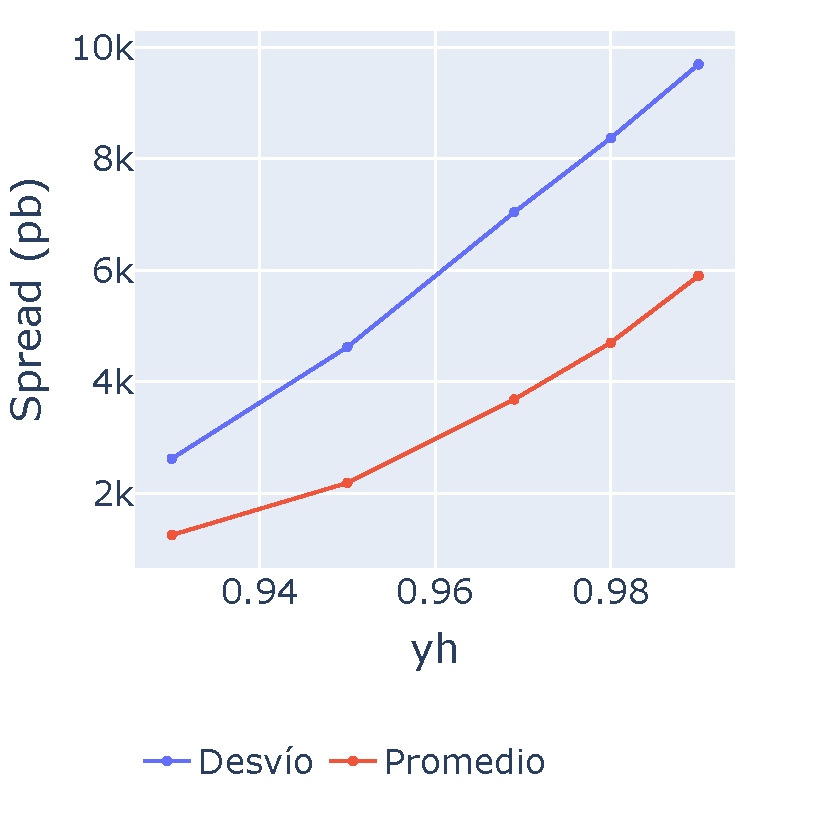
\includegraphics[width=\linewidth]{mom_spread_yh.pdf}\caption{Spread}\end{subfigure}
\begin{subfigure}{.325\textwidth}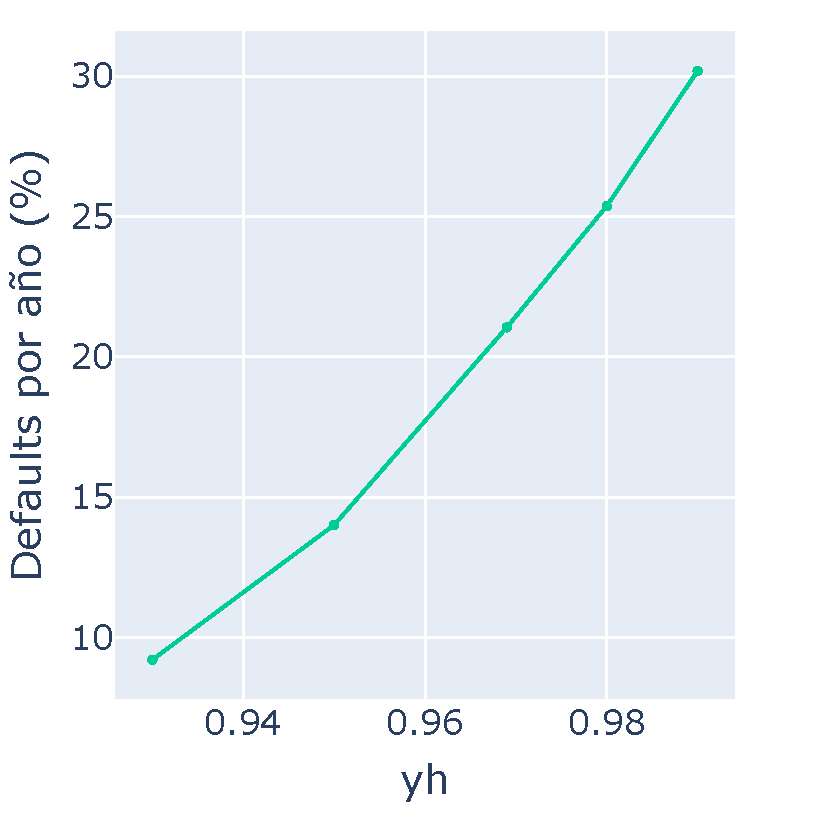
\includegraphics[width=\linewidth]{mom_def_yh.pdf}\caption{Frecuencia de default}\end{subfigure}
\caption{Momentos de la distribución ergódica en función de $y_h$, con $\beta=0.953$.}
\label{fig:momyh}
\end{figure}

\begin{table}[H]
\centering
\begin{tabular}{lcccccc}
\toprule
 & Deuda/PBI & \multicolumn{3}{c}{Spread (puntos básicos)} & Defaults & Tiempo en\\
\cmidrule(lr){3-5}
 & (\%) & Promedio & Desvío & Mediana & por año (\%) & default (\%)\\
\midrule
$y_h=0.93$ & 1.98 & 2053 & 2809 & 1043 & 9.2 & 8.1\\
$y_h=0.95$ & 1.37 & 3054 & 4953 & 1276 & 14.0 & 12.2\\
$y_h=0.969$ (base) & 0.93 & 4656 & 7540 & 1673 & 21.1 & 17.8\\
$y_h=0.98$ & 0.74 & 5746 & 8964 & 1956 & 25.4 & 21.0\\
$y_h=0.99$ & 0.59 & 7031 & 10380 & 2358 & 30.2 & 24.4\\
\bottomrule
\end{tabular}
\caption{Momentos de la distribución ergódica para distintos $y_h$, con $\beta=0.953$.}
\label{tab:momyh}
\end{table}

Un costo de default mayor ($y_h$ menor) aumenta la deuda y reduce el spread y la frecuencia de default, y las cuatro series son monótonas en los cinco valores (Figura~\ref{fig:momyh} y Cuadro~\ref{tab:momyh}). Entre $y_h=0.99$ e $y_h=0.93$, la deuda sube de $0.59\%$ a $1.98\%$ del PBI anual, el spread promedio baja de 7031 a 2053 puntos básicos y la frecuencia de default de $30.2\%$ a $9.2\%$ por año. A diferencia de $\beta$, $y_h$ mueve la región de default. Con $y_h=0.93$, $b^\star(1)=0.223$, contra $0.055$ con $y_h=0.99$. Los acreedores anticipan que al gobierno le cuesta más defaultear y le prestan más barato, de modo que puede sostener más deuda con menos riesgo.

\paragraph{Deuda y spread.} Al variar $\beta$, la deuda y el spread se mueven en la misma dirección, y al variar $y_h$ se mueven en direcciones opuestas. La diferencia está en qué cambia cada parámetro. $\beta$ cambia cuánta deuda quiere el gobierno con precios casi fijos, y más deuda con los mismos precios implica un spread mayor. $y_h$ cambia los precios, porque desplaza la región de default, y con precios más favorables el gobierno se endeuda más y paga menos. Un spread alto no indica por sí solo un país más endeudado.

\subsection{Magnitudes y shocks de preferencias}
\label{sec:momchi}

El Cuadro~\ref{tab:momchi} repite el cálculo de momentos para los tres modelos de la Sección~\ref{sec:chi}, que difieren sólo en $\chi$.

\begin{table}[H]
\centering
\begin{tabular}{lcccccc}
\toprule
 & Deuda/PBI & \multicolumn{3}{c}{Spread (puntos básicos)} & Defaults & Tiempo en\\
\cmidrule(lr){3-5}
 & (\%) & Promedio & Desvío & Mediana & por año (\%) & default (\%)\\
\midrule
$\chi=0.0001$ & 1.04 & 1741 & 1447 & 1434 & 7.9 & 6.5\\
$\chi=0.01$ (base) & 0.93 & 4656 & 7540 & 1673 & 21.1 & 17.8\\
$\chi=0.1$ & 0.47 & 16155 & 14125 & 10478 & 65.3 & 42.4\\
\bottomrule
\end{tabular}
\caption{Momentos de la distribución ergódica para distintos $\chi$, con $\beta=0.953$ e $y_h=0.969$.}
\label{tab:momchi}
\end{table}

Las magnitudes del modelo base son extremas. La deuda es de $0.93\%$ del PBI anual, el spread promedio es de 4656 puntos básicos y el gobierno defaultea en el $21\%$ de los años con acceso al mercado, un default cada cinco años. El promedio del spread está dominado por pocos períodos de spread muy alto (el máximo en una simulación del modelo base es de 43\,574 puntos básicos), y por eso la mediana, 1673, es menos de la mitad.

Una parte de estas magnitudes se debe al shock de preferencias. Con ingreso menor que $y_h$ el default no cuesta ingreso, $v^R$ y $v^D$ quedan cerca, y con $\chi=0.01$ el shock alcanza para decidir el default aun sin deuda. $\mathcal P(0,y)$ vale $0.296$ en $y=0.858$ y $0.18$ en $y=0.926$. El precio de una emisión casi nula ya incluye ese riesgo (con $y=1$, $q=0.977$ contra $0.983$), y el spread se registra aunque el gobierno emita muy poca deuda. Con $\chi=0.0001$ esas probabilidades son nulas, y el spread promedio cae a 1741 puntos básicos y la frecuencia de default a $7.9\%$ por año (Cuadro~\ref{tab:momchi}). Con $\chi=0.1$ suben a 16\,155 puntos básicos y $65.3\%$.

El resto se explica por el costo de default. Aun sin shocks, con ingreso por debajo de $y_h$ el único costo de defaultear es la exclusión, y el gobierno defaultea con casi cualquier deuda ($b^\star(0.858)=0.002$ con $\chi=0.0001$). Por eso los defaults se concentran en recesiones. En una simulación del modelo base el ingreso promedio es $0.929$ en los períodos de default y $1.011$ en los de repago.

\paragraph{Conclusión.} El modelo genera mucho riesgo con muy poca deuda. La deuda no supera el $2\%$ del PBI anual en ningún caso, y el spread promedio va de 1741 a 16\,155 puntos básicos. La paciencia y el costo de default mueven los momentos por canales distintos. La paciencia cambia cuánta deuda elige el gobierno con precios casi fijos, y la deuda y el spread se mueven juntos. El costo de default cambia los precios, y un costo mayor trae más deuda y menos spread. Una parte grande del riesgo viene del shock de preferencias, que con $\chi=0.01$ genera defaults aun sin deuda cuando el ingreso es menor que $y_h$.

\end{document}
